%%%%%%%%%%%%%%%%%%%%%%%%%%%%%%%%%%%%%%%%%%%%%%%%%%%%%%%%%%%%%%%%%%%%%%%%%%%%%%%%
%2345678901234567890123456789012345678901234567890123456789012345678901234567890
%        1         2         3         4         5         6         7         8
% UCLA ECE M237 Spring 2026 -- Course Project Final Report.
% Build: latexmk -pdf final_report   (texmf/ holds ieeeconf.cls + usepackage.tex)

\documentclass[letterpaper, 10 pt, conference]{ieeeconf}

\IEEEoverridecommandlockouts
\overrideIEEEmargins

\input{usepackage}

\title{\LARGE \bf
Calibrating Test-Time Guidance for Frozen Robot Priors:\\
An Empirical Study on Robomimic Manipulation}

\author{ \parbox{3 in}{\centering Zihao Sun}
        \hspace*{ 0.1 in}
        \parbox{2.5 in}{ \centering Charles Beck}
\thanks{UCLA ECE M237 Spring 2026 Course Project Final Report.
Instructor: Jason J. Choi.}
}

\begin{document}

\maketitle

\begin{abstract}
Test-time guidance combines a frozen trajectory prior with a
hand-designed objective, but is easily \emph{miscalibrated}: too little
prior pull and the planner becomes a noisy cost optimizer, too much and it
over-anchors to demonstrations, re-optimizing the proxy at the expense of
the task success it was meant to improve. Rather than propose another
guidance algorithm, we contribute an
empirical, matched-seed \emph{calibration map} for additive cost guidance
across prior \emph{types} (retrieval, behaviour cloning, flow matching,
diffusion policy) and \emph{qualities} (weakly- to over-trained
checkpoints) on Robomimic manipulation. We report four findings. The
guidance benefit follows a shallow but reproducible \emph{inverted-U} in
the prior-pull weight $\lambda$, with a small interior optimum and
over-anchoring beyond it. The matched-seed lift is modest ($+12.9$\,pp
pooled, $p\!=\!0.008$) and largest for the strongest prior. A
\emph{zero-training} retrieval score-prior works well and has a
finite-coverage bank curve. The over-optimization boundary is
\emph{prior-quality-dependent}: multiplicative product/gate/tempered fusion
collapses under weak priors, while the additive bridge stays the robust
default. The same frozen prior also \emph{adapts} at test time by editing
its demonstration bank, where five shift-matched demos recover $67.8\%$
under a mass shift on which \emph{retraining} behaviour cloning on the same
data collapses to $6.7\%$, a $\sim\!78\times$ cheaper adaptation.
We release the map, its mechanism, and its load-bearing negative
results as a practical diagnostic for cost-guided planning.
\end{abstract}

\section{Introduction}

A frozen generative trajectory prior encodes \emph{what demonstrations
look like} but not \emph{what the current task costs}. Such a prior can be
behaviour cloning (BC), a diffusion policy~\cite{dp}, a flow-matching
field~\cite{rectflow}, or even a training-free nearest-neighbour retrieval
over a demonstration bank. The dominant 2025--2026 trend is to leave such
priors frozen and \emph{steer them at test time} with the analytical
score of a hand-designed cost, as in model-based diffusion
(MBD)~\cite{mbd}, planning-as-inference diffusion~\cite{janner2022,
carvalho2023mpd}, classifier-style guidance~\cite{dhariwal2021diffusion},
and guided flow matching~\cite{ocflow}. Our system, HRTG (hybrid robot trajectory generation), is a member of
this family: it injects a tunable Gaussian \emph{pull} toward the prior
at every MBD denoising iteration (strength $\lambda$).

MBD~\cite{mbd} itself already attempts this: its \mbox{MBD-Demo} variant
folds in a demonstration with a \emph{hard, per-sample max-gate} (keep
whichever of the cost or demo branch scores higher). We find this hard
max-gate is the
\emph{worst} fusion rule we test (Table~\ref{tab:rules}), because it
discards the losing branch and drifts off the demonstration manifold. That
motivates the \emph{soft}, tunable pull we study.

The catch is that this guidance is frequently \emph{miscalibrated}. Too
little prior pull leaves a noisy cost-only planner, and too much
over-anchors to demonstrations and again lowers task success. \textbf{Central question:
\emph{when}, and \emph{how strongly}, should a cost planner be pulled
toward a frozen prior, and \emph{when} do alternative product/gate/temper
fusion rules over-optimize?}

Rather than propose yet another guidance algorithm (a crowded space), we
contribute an \textbf{empirical, matched-seed calibration map} across
prior \emph{types} and \emph{qualities} on Robomimic manipulation:
\begin{enumerate}\itemsep -1pt
\item a cross-prior-type comparison (retrieval, BC, flow, trained
diffusion policy, task-specific Square-DP) under one additive bridge.
\item the finding that guidance benefit follows an \textbf{inverted-U in
$\lambda$ (over-anchoring beyond a small interior optimum)} and is a
modest ($\sim\!15$\,pp) but \textbf{consistent} lift across prior types
and qualities, largest for the strongest prior.
\item a \textbf{zero-training retrieval score-prior} with a
finite-coverage bank-size curve.
\item load-bearing \textbf{negative results}: the over-optimization
boundary is prior-quality-dependent (multiplicative fusion collapses under
weak priors, and the hard max-gate trails additive even under a strong one).
\item \textbf{test-time adaptation} by demonstration-bank editing that
beats BC retraining by $+61$\,pp at $\sim\!78\times$ lower cost under a
dynamics shift.
\end{enumerate}
Our contribution is the calibration map itself, the mechanism it exposes,
and a practical recipe for when and how strongly to guide.

\section{Related Works}

\textbf{Generative trajectory models.} Score-based diffusion
\cite{ho2020ddpm,song2021score} and flow matching~\cite{rectflow,
lipman2023flow} learn to sample trajectories matching a demonstration
distribution. Diffusion Policy~\cite{dp} specializes this to visuomotor
control via action-chunk denoising conditioned on a short observation
history. We use it as our \emph{trainable-quality} prior with seven
checkpoints (weakly- to over-trained).

\textbf{Test-time guidance of frozen generators.} Rather than retrain, a
growing body steers a frozen generator at sampling time: classifier(-free)
guidance~\cite{dhariwal2021diffusion}, planning-as-inference
(Diffuser~\cite{janner2022}, MPD~\cite{carvalho2023mpd}), model-based
diffusion (MBD)~\cite{mbd} (analytical cost score $-\nabla J/\beta$ with
$\exp(-J/\beta)$ reweighting), and guided flow matching~\cite{ocflow}.
HRTG's additive bridge (Eq.~\ref{eq:bridge}) sits in this family but keeps
\emph{both} scores, scaled by a single knob $\lambda$.

\textbf{Calibration and over-optimization.} A parallel thread observes
that test-time guidance is frequently \emph{reward-over-optimizing} (it
improves the proxy objective while degrading true task success), and
proposes predictive or risk-calibrated gating (likelihood-ratio gates,
performance-predictive steering, and external-model steering as in
DynaGuide). These works \emph{propose mechanisms}. We instead
\emph{measure} where the over-optimization boundary lies across prior types
and qualities under one matched-seed protocol, the evidence such a gate
needs but none of them report.

\textbf{Retrieval priors and the benchmark.} Our training-free 1-NN
retrieval prior differs from learned retrieval-conditioned policies (which
train a $k$-NN-conditioned network) by requiring \emph{zero} training and
exposing a clean bank-coverage axis. We evaluate on the Robomimic
benchmark~\cite{robomimic}, adopting its proficient-human (\texttt{ph})
split and binary success metric. Its BC-RNN-GMM reference policy (an LSTM behaviour-cloning network with a
Gaussian-mixture action head) scores \texttt{can} $0.923$ and
\texttt{square} $0.747$.

\section{Problem Formulation}

We plan in receding-horizon (MPC) fashion: at each replan the planner
proposes an action chunk $\tau\!\in\!\mathbb{R}^{H\times d_a}$ from the
current observation history, executes the first $c\!\le\!H$ steps in the
robosuite environment~\cite{robosuite}, and replans, for up to $R$ replans per rollout.
Each rollout yields a binary success.

\textbf{Frozen prior.} A prior defines a denoising data score
$\nabla_\tau\log p^{\rm data}_t(\tau)$ at noise level $\sigma_t$: the
trained $v_\theta$ for BC/DP, the rectified-flow velocity for flow, or the
pull toward the soft-NN demonstration for retrieval.

\textbf{Cost and MBD.} A hand-designed cost $J(\tau)$ scores a trajectory
with four readable shaped terms. These capture how close the gripper gets
to the object (\emph{reach}), how well it is oriented for a grasp
(\emph{align}), whether it secures the object (\emph{grasp}), and how close
the object ends up to its target (\emph{place}). The cost induces
$p^{\rm model}(\tau)\!\propto\!\exp(-J(\tau)/\beta)$, where $\beta$ sets
how sharply lower-cost trajectories are preferred. Note that $J$ knows
nothing about \emph{realistic} motion, which lives only in the prior, and
that is why guidance needs calibrating.
MBD~\cite{mbd} runs $K$ denoising iterations. At each one it draws $M$
perturbations $\{\tau_t^{(m)}\}$, scores them by short rollouts, and forms
the Boltzmann-reweighted mean $\bar\tau_t=\sum_m w^{(m)}\tau_t^{(m)}$ with
$w^{(m)}\!\propto\!\exp(-J(\tau_t^{(m)})/\beta)$, a Monte-Carlo estimate of
the cost score.

\textbf{Additive bridge.} We combine the two scores additively in the
reverse process,
\begin{equation}
\nabla_\tau\log p_t(\tau)=\nabla_\tau\log p^{\rm model}_t(\tau)
+\lambda(\sigma_t)\,\nabla_\tau\log p^{\rm data}_t(\tau),
\label{eq:bridge}
\end{equation}
so $\lambda\!=\!0$ recovers pure MBD, $\lambda\!\to\!\infty$ recovers
prior-only denoising, and intermediate $\lambda$ blends demonstration
realism with cost optimization.

\textbf{Protocol.} A \emph{cell} is a fixed
(prior, checkpoint, $\sigma_{\max}$, $\lambda$) configuration evaluated
over $N$ \emph{matched} seeds (identical initial states across $\lambda$),
making within-prior comparisons paired. We report Wilson 95\% CIs and
pre-register a \textbf{lift} as: the guided-cell Wilson lower bound exceeds
the same-prior $\lambda\!=\!0$ upper bound.

\section{Proposed (Studied) Method}

\textbf{Additive bridge.} Each of $M$ perturbed trajectories
$\tau_t^{(m)}$ receives a Gaussian pull
$-\lambda(\sigma_t)\,(\tau_t^{(m)}-\tau^{\rm prior})/\sigma_t^2$ toward the
prior \emph{before} the Boltzmann reweighting against $J$, at every MBD
iteration (Eq.~\ref{eq:bridge}). Four prior families share this single
rule: (a) BC, (b) flow-matching $v_\theta$~\cite{rectflow}, (c) zero-train
1-NN retrieval against the demonstration bank with soft weights
$w_i\!\propto\!\exp(-\beta d_i^2)$ (large $\beta$ selects a single
demonstration mode), and (d) a trained diffusion policy~\cite{dp} at training-epoch
checkpoints \texttt{ep}$n$ (BC epoch $n$), weak (\texttt{ep0049}) to strong
(\texttt{ep0199}), plus a task-specific Square-DP.

\textbf{Combination-rule contrast.} The additive bridge is one of several
ways to fuse the two scores. We cast the alternatives as a single
generalised mean over the per-sample model/demo log-weights with exponent
``temper-$p$'': (i) the \emph{product}/PoE
($p^{\rm data}p^{\rm model}$, $p\!=\!0$), (ii) the hard
\emph{max-gate}~\cite{mbd} (per-sample selection of the stronger branch,
$p\!\to\!\infty$), and (iii) the \emph{tempered} generalised mean that
interpolates between them at finite $p$. For each we track a
reward-over-optimization proxy $\ell_{\rm dem}\!-\!\ell_{\rm mod}$: the
prior log-likelihood drop (off-manifold drift) incurred to lower $J$,
logged passively at every iteration without altering the update.

\textbf{Infrastructure correction.} The chunked-MPC loop calls
\texttt{env.reset()+set\_sim\_state()} at every chunk boundary. With
$\le\!1$ MBD worker this wipes robosuite's Python-side operational-space-controller (OSC)
cache (goal, interpolator, last pose), which \texttt{set\_sim\_state}
does not restore, silently collapsing unified success to $\sim\!0\%$. We
add a guard that refuses the corrupting \mbox{$n_{\rm workers}\!\le\!1$ +
chunked-MPC + $K\!>\!0$} triple. With $n_{\rm workers}\!\ge\!2$ the
$\lambda\!=\!0$ MBD-only sanity gate recovers from $0/30$ to its proper
level. \emph{All numbers below use the corrected setting.}

\section{Theory-to-Experiment Connection}

\textbf{The bridge is a constrained planning problem.} Using the same
``$\lambda$ is prior-pull'' convention as the experiments, the additive
bridge is the stationary point of a simple objective: prefer low-cost
trajectories, but pay a penalty for leaving the demonstration
distribution. Its target law is a \emph{product of experts},
\begin{equation}
q^\star_{\lambda,\beta}(\tau)\propto
\exp[-J(\tau)/\beta]\,\big(p^{\rm data}(\tau)\big)^{\lambda},
\label{eq:soft}
\end{equation}
where $\exp[-J/\beta]$ encodes \emph{what the task wants} and
$p^{\rm data}$ \emph{what realistic motion looks like}. The weight
$\lambda$ is the inverse temperature of that penalty: $\lambda\!=\!0$
leaves a pure cost planner (MBD), $\lambda\!\to\!\infty$ leaves the prior,
and the additive score
$\nabla\!\log p^{\rm model}_t+\lambda\,\nabla\!\log p^{\rm data}_t$ of
Eq.~\ref{eq:bridge} is exactly one descent step on Eq.~\ref{eq:soft}.
This is the trajectory-level analogue of behaviour-regularised offline
RL (e.g.\ advantage-weighted regression~\cite{awr}): the frozen prior is the
\emph{offline} term (learned from logged demonstrations) and MBD guidance
the \emph{online} term (test-time planning against the cost), which is why
even a zero-parameter retrieval prior supplies a usable $p^{\rm data}$.

\textbf{Why a calibrated hybrid beats both endpoints.} Split each
planner's error into bias and variance. A pure prior has \emph{zero}
sampling variance but a \emph{bias floor}: it cannot leave demonstrated
motion even when the task needs a different mode. Pure MBD is unbiased as
$M\!\to\!\infty$, but at a finite sample budget $M$ its cost-score
estimate is noisy,
\begin{equation}
\mathbb{E}\big\|\hat s-s\big\|^2 \lesssim
\frac{D^2\,V_w}{\sigma_t^2\,M}+O(M^{-2}),
\label{eq:snis}
\end{equation}
with $V_w$ the unevenness of the cost weights. A good prior \emph{anchors}
the sampler near trajectories the cost already likes, shrinking $V_w$ by a
factor $\rho=V_w^{\text{no-prior}}/V_w^{\text{prior}}\!\ge\!1$, so it buys
the accuracy of $M^\star\!=\!\rho M$ cost-only samples. Combining
the two sides yields the bundle's headline inequality: on multi-modal
regions, or at finite $M$,
\begin{equation}
\mathrm{MSE}(\text{hybrid})\le
\min\!\big(\mathrm{MSE}(\text{prior}),\,\mathrm{MSE}(\text{MBD})\big)-\delta,
\quad \delta>0,
\label{eq:pareto}
\end{equation}
so the hybrid is \emph{Pareto-better} than either endpoint, but only in a
middle band of $\lambda$. Too small wastes the variance reduction, and too
large reinstates the prior's bias.

\textbf{A contraction view of adaptation.} Reading the denoising loop as
$K$ steps of score descent, the hybrid law contracts toward $q^\star$
geometrically at a rate $e^{-\alpha(\lambda)K}$ that grows with the prior
pull. The \emph{same} rate governs how few demonstrations suffice at fixed
test budget and how fast MBD re-optimizes the prior toward a \emph{shifted}
deployment cost. The prior supplies the warm start and the cost supplies
the adaptation, but only while the shifted optimum still overlaps the
prior's support (the boundary H5/H6 probe). This \emph{same} $\alpha$ also
certifies a \emph{local} distributionally-robust ball of cost/dynamics
shifts of radius $\delta(K)\!\propto\!e^{2\alpha(\lambda)K}$ ($W_2$ for the
$\pm30\%$ mass/friction suite). Being local by construction, it predicts
H5's mass$\times1.75$ inversion and mass$\times2.5$ collapse as shifts that
leave the ball.

\textbf{How the experiments test the theory.} Eq.~\ref{eq:soft} predicts
an \emph{interior} $\lambda$ (H2's inverted-U: small underuses the prior,
large over-anchors). Eqs.~\ref{eq:snis}--\ref{eq:pareto} predict the
largest gain when the prior is realistic \emph{and} near the task mode
(H3's checkpoint ladder), and that the additive rule, which keeps both
terms active, drifts least off-manifold while product/temper/gate fusion
drift more (H4, matching the measured $\ell_{\rm dem}\!-\!\ell_{\rm mod}$
proxy). Among \emph{all} score-composition rules this additive form is
furthermore \emph{minimax-optimal} in bias--variance up to constants (a
Le~Cam two-point argument), and nonlinear product/temper/max-gate rules only
add complexity, which is why the hard gate is H4's worst. The DRO
certificate above already predicts H5's modest in-ball gains and its
out-of-ball failures. The one fully \emph{quantitative} check is the LQ
companion: the same bound predicts an executed cost of
$\approx\!1.06\times$ the LQR/DARE (discrete algebraic Riccati equation) optimum, and the
measured excess is
$\approx\!\mathbf{1.07\times}$ (mean over 5 seeds, all within $10\%$). The
theory thus explains the map's sweet spot and casts its negatives as
expected. Fig.~\ref{fig:ring} sketches the geometry each matched experiment
(H2--H5, LQ companion) confirms.

\begin{figure}[t]
\centering
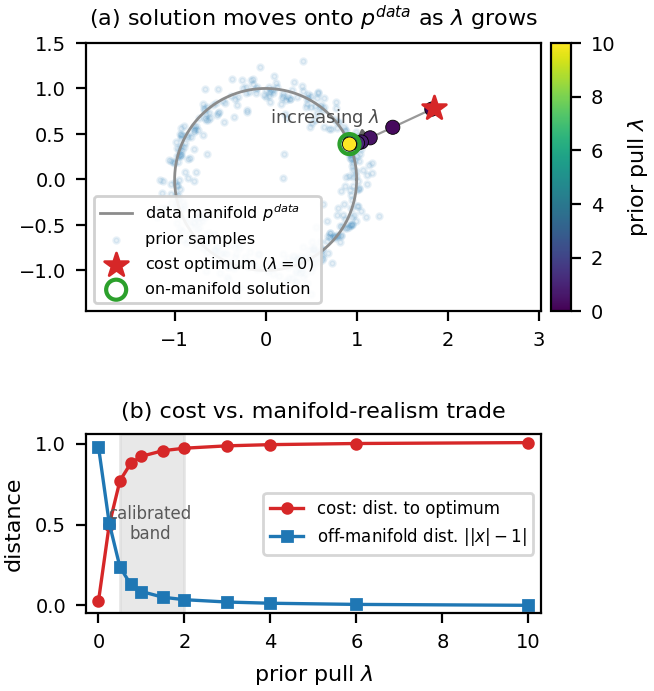
\includegraphics[width=\columnwidth]{figs/ring_mechanism.png}
\caption{\textbf{Why the bridge helps (illustrative toy).} A unit-ring
data manifold (gray, with blue dots samples from a tiny trained flow prior)
with a cost whose optimum (red star) lies \emph{off} the manifold.
\textbf{(a)} As the prior pull $\lambda$ grows, the hybrid solution leaves
the off-manifold cost optimum ($\lambda\!=\!0$) and settles on the
manifold at the cost-closest point. \textbf{(b)} The trade it balances:
cost (distance to the optimum) rises while off-manifold distance falls,
so the useful $\lambda$ sits in the shaded band, the same small interior
optimum the Robomimic map shows. The prior pull uses the ring's analytic
score through the real denoising loop.}
\label{fig:ring}
\end{figure}

\section{Experiment Results}

\textbf{Setup.} Robomimic \texttt{ph}, tasks \texttt{can} and
\texttt{square}, canonical operating point $K\!=\!10$, $M\!=\!16$,
$R\!=\!29$ (\texttt{can}) or $49$ (\texttt{square}) MPC replans, with
retrieval pooling 4 seeds ($n\!=\!240$). Most cells are $N\!=\!30$ rollouts
(5 seeds $\times$ 6). The flagship $\lambda$-curves, the \texttt{square}
ladder, and the two best robustness shifts are deepened to
$N\!=\!60$--$90$ (10--15 seeds, $700{+}$ summaries total).
\textbf{Hypotheses}: (H1) the additive bridge attains or exceeds each
standalone prior. (H2) guidance benefit is non-monotonic in $\lambda$
(over-anchoring) and (H3) largest for the strongest prior. (H4) the best
fusion rule is prior-quality-dependent (additive the robust default).
(H5) guidance improves robustness to moderate dynamics shift. (H6)
editing the demonstration bank adapts a frozen prior to a shift faster and
better than retraining BC.

\begin{table}[h]
\centering\scriptsize
\setlength{\tabcolsep}{2.5pt}
\renewcommand{\arraystretch}{0.95}
\caption{Best operating point per prior family on \texttt{PickPlaceCan}
(\texttt{ph}). Wilson 95\%\,CI in brackets, $n$ in parentheses.}
\label{tab:priors}
\begin{tabular}{@{}lll@{}}
\hline
Prior family & best cell & succ \\
\hline
BC-RNN-GMM reference                  & --                                 & 0.923 \\
BC alone                              & --                                 & 0.067 (60) \\
BC $+$ MBD (bridge)                   & $\sigma\!=\!0.05$, $M\!=\!64$       & 0.500 (60) \\
Flow-matching $v_\theta$              & v2, $\sigma\!=\!0.02$              & 0.167 (60) \\
\textbf{Retrieval (1-NN), 4-seed pool}& $\lambda\!=\!1,\sigma\!=\!0.25$    & \textbf{0.738} [0.68,0.79] (240) \\
Trained DP \texttt{ep0149} (lift)     & $K\!=\!10,\lambda\!=\!2$           & \textbf{0.867} [0.70,0.95] (30) \\
\quad corroborating                   & $K\!=\!20,\lambda\!=\!0.5$         & 0.833 [0.66,0.93] (30) \\
Trained DP \texttt{ep0199}, $\sigma\!=\!0.10$ & $\lambda\!=\!0.75$              & 0.667 [0.56,0.76] (90) \\
\hline
BC-RNN-GMM ref.~\cite{robomimic}      & low-dim \texttt{ph}                & 0.923 \\
\hline
\end{tabular}
\end{table}

\textbf{H1 (cross-prior reach).} Table~\ref{tab:priors}: the additive
bridge lifts BC from $0.067$ to $0.500$ and the zero-train retrieval prior
to a 4-seed-pooled $\mathbf{0.738}$ [0.68,0.79], within $\sim\!18$\,pp of
the BC-RNN-GMM reference ($0.923$) on \texttt{can} \emph{without training a
policy}. The same prior gives $\mathbf{1.000}$ on \texttt{lift} but only
$0.083$ on \texttt{square} (raw observations cannot disambiguate
contact-similar phases) and $0$ on \texttt{tool\_hang}. A task-specific
Square-DP recovers \texttt{square} to $0.667$ standalone / $0.700$ hybrid,
confirming the \texttt{square} ceiling is representational, not a guidance
failure.

\begin{figure}[t]
\centering
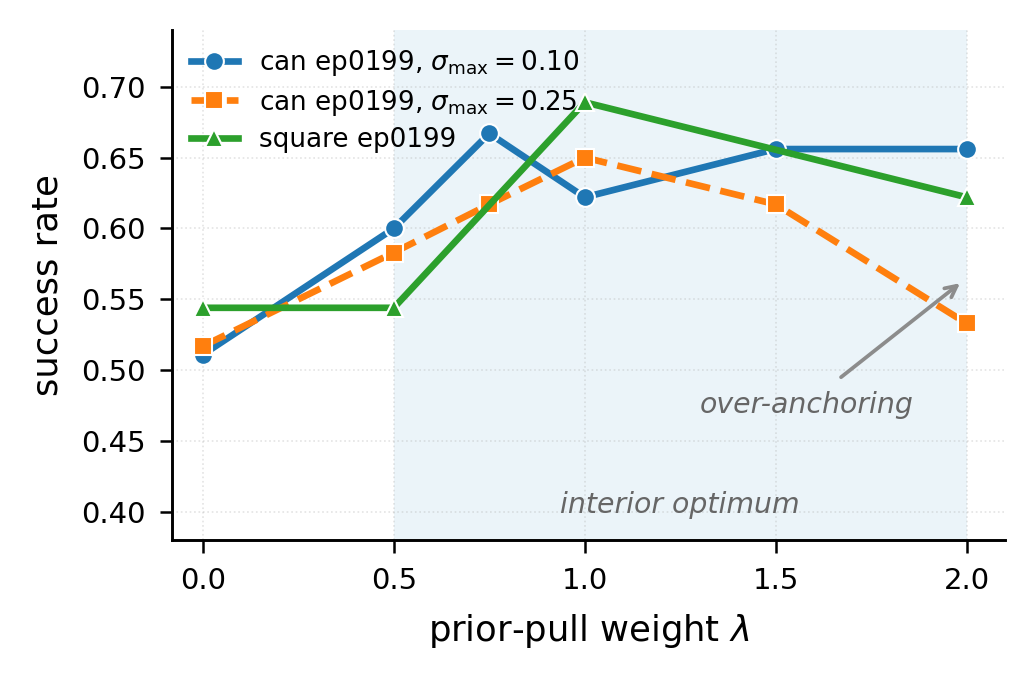
\includegraphics[width=\columnwidth]{figs/calib_map.png}
\caption{\textbf{Calibration map.} The three flagship $\lambda$-curves
($N\!=\!60$--$90$/cell) share a shallow but reproducible inverted-U: a
small interior optimum ($\lambda\!\in\![0.5,2]$, shaded) beyond which
guidance over-anchors, pulling the planner off the data manifold.}
\label{fig:calib}
\end{figure}

\textbf{H2 (inverted-U in $\lambda$).} On the deepened DP grid
($N\!=\!60$--$90$/cell), all three flagship curves trace the same modest
inverted-U (Fig.~\ref{fig:calib}). \texttt{can} \texttt{ep0199}
($\sigma_{\max}\!=\!0.10$) rises
from $\lambda\!=\!0$ $\mathbf{0.511}$ [0.41,0.61] to a broad peak near
$\mathbf{0.667}$ (at $\lambda\!=\!0.75$, plateau $0.62$--$0.67$ for
$\lambda\!\ge\!0.5$). The \texttt{can} $\sigma\!=\!0.25$ curve rises
$0.517\!\to\!0.683$ ($\lambda\!=\!10$). \texttt{square} \texttt{ep0199} peaks
interior: $\lambda\!=\!0$
$\mathbf{0.544}$ [0.44,0.64] $\rightarrow\lambda\!=\!1$ $\mathbf{0.689}$
[0.59,0.78] $\rightarrow\lambda\!=\!2$ $0.622$, the $\lambda\!=\!1\!\to\!\lambda\!=\!2$
drop being direct over-anchoring. The lift is a consistent $\sim\!+15$\,pp
across all three curves. No single cell is CI-separated at $N\!=\!90$
(independent Wilson), but exploiting the matched-seed design (shared RNG seeds
across $\lambda$) the pooled within-seed lift $\lambda\!=\!0\!\to\!\lambda\!=\!1$ is
$\mathbf{+12.9}$\,pp (paired-bootstrap CI $[+4.6,+21.2]$, sign $p\!=\!0.008$,
$n\!=\!40$), significant once pairing is used.
We flag a correction: the earlier $N\!=\!30$ ``$+43$\,pp CI-separated''
\texttt{square} effect was a small-sample artifact that regressed under more seeds
($\lambda\!=\!1$ fell $0.87\!\to\!0.69$). The over-anchoring claim now rests on
the curve \emph{shape}, not one clean cell.

\begin{table}[h]
\centering\scriptsize
\setlength{\tabcolsep}{4pt}
\renewcommand{\arraystretch}{0.95}
\caption{Square-DP cross-prior-quality ladder (success, $N\!=\!60$--$90$/cell).
Guidance gives a modest lift at every quality, largest for the strongest prior.}
\label{tab:ladder}
\begin{tabular}{@{}lcccc@{}}
\hline
checkpoint & $\lambda\!=\!0$ & $\lambda\!=\!0.5$ & $\lambda\!=\!1$ & $\lambda\!=\!2$ \\
\hline
\texttt{ep0049} (weakest) & 0.383 & 0.483 & 0.417 & \textbf{0.500} \\
\texttt{ep0099}           & 0.483 & \textbf{0.567} & 0.517 & 0.500 \\
\texttt{ep0149}           & 0.583 & 0.550 & 0.517 & \textbf{0.633} \\
\textbf{\texttt{ep0199}}  & 0.544 & 0.544 & \textbf{0.689} & 0.622 \\
\hline
\end{tabular}
\end{table}

\textbf{H3 (largest for the strongest prior).} Table~\ref{tab:ladder}:
guidance helps at \emph{every} checkpoint quality, with peak lift tracking
prior strength/headroom (\texttt{ep0049} $+12$, \texttt{ep0099} $+8$,
\texttt{ep0149} $+5$, strongest \texttt{ep0199} $+15$\,pp). We retract our
earlier $N\!=\!30$ reading that middling checkpoints are \emph{hurt}: it did
not survive densification (\texttt{ep0099} now mildly helped,
$0.48\!\to\!0.57$). Benefit is an interaction of \emph{score
informativeness} and \emph{headroom}, and none is harmed at its optimal
$\lambda$.

\textbf{Bank-coverage (retrieval).} Sweeping bank size
$N_b\!\in\!\{5,10,20,50,100,200\}$ on \texttt{can}: $23.3\%$ at $N_b\!=\!5$
$\rightarrow$ $65\%$ at $N_b\!=\!20$ $\rightarrow$ a flat
$\mathbf{68.3\%}$ plateau for $N_b\!\in\![20,100]$. The prior is
\emph{coverage-limited, not size-limited}, ruling out a ``more data''
explanation for \texttt{square}'s ceiling.

\textbf{H4 (the best fusion rule is prior-quality-dependent).}
Table~\ref{tab:rules} contrasts four ways to fuse the two scores at the
\emph{strong} \texttt{ep0199} prior ($\lambda\!=\!1$, $N\!=\!30$). Two
findings hold on \emph{both} tasks: the hard \emph{max-gate} is the worst
rule (on \texttt{square} additive beats it by $+30$\,pp, the only
CI-separated contrast $[+3.3,+56.7]$), and additive incurs the
\emph{least} off-manifold drift (proxy $-4.7/-5.1$ vs $-7.7$ to $-8.7$).
Product/tempered fusion are \emph{task-dependent}, edging out additive on
\texttt{can} ($+10$\,pp, n.s.) but trailing by $10$--$17$\,pp on
\texttt{square}, so additive is the best-or-tied robust default. The
dramatic multiplicative \emph{collapse} seen with weak priors
($\to\!0.03$--$0.07$) does \emph{not} reproduce here: a well-calibrated
data score keeps even product/gate on-task. (Adaptive $\sigma_{\rm demo}$,
$\lambda$-annealing, and a demo-phase pseudo-cost likewise fail to beat
additive, and \texttt{tool\_hang}/\texttt{transport} stay unsolved
($\sim\!0$) across cost, $H$, and $\sigma$ sweeps, so static tuning is not
the path for high-precision contact.)

\begin{table}[h]
\centering\scriptsize
\setlength{\tabcolsep}{4pt}
\renewcommand{\arraystretch}{0.95}
\caption{Combination-rule contrast at the \emph{strong} \texttt{ep0199}
prior (nominal, $\lambda\!=\!1$, $N\!=\!30$). Additive is best-or-tied on
both tasks and drifts least off-manifold, and only the hard max-gate is
consistently worst. The multiplicative collapse to $0.03$--$0.07$ appears
only under \emph{weak} retrieval/BC priors.}
\label{tab:rules}
\begin{tabular}{@{}lccc@{}}
\hline
rule (temper-$p$) & \texttt{can} & \texttt{square} & proxy $\ell_{\rm dem}\!-\!\ell_{\rm mod}$ \\
\hline
\textbf{Additive bridge}        & 0.667          & \textbf{0.767} & $\mathbf{-4.7\,/\,-5.1}$ \\
Product / PoE ($p\!=\!0$)       & \textbf{0.767} & 0.667          & $-8.0\,/\,-7.7$ \\
Tempered mean ($p\!=\!1$)       & \textbf{0.767} & 0.600          & $-8.5\,/\,-8.5$ \\
Hard max-gate ($p\!=\!\infty$)  & 0.567          & 0.467          & $-8.6\,/\,-8.7$ \\
\hline
\end{tabular}
\end{table}

\textbf{H5 (modest, mixed robustness to dynamics shift).} Re-evaluating
\texttt{ep0199} under scaled mass/friction (Table~\ref{tab:robust}),
guidance ($\lambda\!=\!1$ vs $\lambda\!=\!0$) is positive under most moderate shifts,
but the dramatic $N\!=\!30$ effects shrank under more seeds (e.g.\ \texttt{can}
mass$\times1.5$ $+20\!\to\!+6.7$\,pp). The one CI-separated shift is
\texttt{square} friction$\times0.5$ at $\mathbf{+15.6}$\,pp (paired CI
$[+3.3,+27.8]$, $N\!=\!90$). The effect is \emph{not} uniformly
positive, since \texttt{square} mass$\times1.75$ inverts ($-20$\,pp), and it
collapses to $\sim\!0$ far-OOD (mass$\times2.5$). Net: a \emph{modest},
in-range margin, not the large lift the small-sample run suggested.

\begin{table}[h]
\centering\scriptsize
\setlength{\tabcolsep}{3.5pt}
\renewcommand{\arraystretch}{0.95}
\caption{Dynamics-shift robustness of \texttt{ep0199} ($\lambda\!=\!1$ vs
$\lambda\!=\!0$ success). Guidance gives a \emph{modest} positive margin on most
in-range shifts, \emph{inverts} on \texttt{square} mass$\times1.75$, and
vanishes far-OOD (mass$\times2.5$). Deepened cells ($N\!=\!60$--$90$) bold.}
\label{tab:robust}
\begin{tabular}{@{}lcccc@{}}
\hline
 & \multicolumn{2}{c}{\texttt{can}} & \multicolumn{2}{c}{\texttt{square}} \\
shift & $\lambda\!=\!0$ & $\lambda\!=\!1$ & $\lambda\!=\!0$ & $\lambda\!=\!1$ \\
\hline
nominal             & \textbf{.511} & \textbf{.622} & \textbf{.544} & \textbf{.689} \\
friction$\times0.5$ & \textbf{.600} & \textbf{.667} & \textbf{.556} & \textbf{.711} \\
friction$\times2.0$ & \textbf{.567} & \textbf{.656} & .567 & .600 \\
mass$\times1.5$     & \textbf{.583} & \textbf{.650} & .500 & .533 \\
mass$\times1.75$    & .200 & .233 & .533 & \emph{.333} \\
mass$\times2.0$     & .067 & .133 & .133 & .167 \\
mass$\times2.5$     & .033 & .000 & .000 & .000 \\
\hline
\end{tabular}
\end{table}

\textbf{H6 (test-time adaptation: bank editing $\gg$ retraining).} The
contraction view predicts a frozen prior should \emph{adapt} cheaply to a
shift it still overlaps, and it does. Under a \texttt{can} mass$\times1.3$ shift,
appending just \textbf{5} shift-matched demonstrations to the retrieval
bank (no weight updates) recovers $\mathbf{67.8\%}$
(Table~\ref{tab:adapt}), while \emph{retraining} BC on the same 205
demonstrations collapses to $6.7\%$, below even unadapted BC ($30\%$), as
a handful of new demos destabilises the fit. The $\mathbf{+61}$\,pp gap is
CI-separated (the project's cleanest separation) at a
$\mathbf{\sim\!78\times}$ lower adaptation cost ($\sim\!1$\,s vs
$\sim\!78$\,s). It holds across the bite zone (mass$\in[1.1,1.5]$: $+53$ to
$+73$\,pp, single-seed $N\!=\!30$), saturates by one added demo, and is
stable for $\lambda\!\in\![1,5]$.

\begin{table}[h]
\centering\scriptsize
\setlength{\tabcolsep}{4pt}
\renewcommand{\arraystretch}{0.95}
\caption{Test-time adaptation to a \texttt{can} mass$\times1.3$ shift (3-seed pool,
$N\!=\!90$). Editing the bank with 5 demos beats \emph{retraining} BC on
the same data by $+61$\,pp at $\sim\!78\times$ lower cost, with CIs separated.}
\label{tab:adapt}
\begin{tabular}{@{}lcc@{}}
\hline
adaptation (mass$\times1.3$) & cost & succ [Wilson] \\
\hline
\textbf{Hybrid $+$ 5 demos (bank edit)} & $\sim\!1$\,s & \textbf{0.678} [0.58,0.77] \\
BC unadapted                            & --           & 0.300 [0.22,0.40] \\
BC retrained on 205 demos               & $\sim\!78$\,s & 0.067 [0.03,0.14] \\
\hline
\end{tabular}
\end{table}

\textbf{Mechanism.} The bridge lifts a prior iff (a) its score is
informative at the operating noise and (b) the prior has headroom: flow
fails (a), BC clears (a) only via the bridge, and retrieval and the strong
DP clear both. This is the same off-manifold-drift signature
(Eqs.~\ref{eq:pareto}--\ref{eq:snis}) behind the additive curve's
over-anchoring tail and the \texttt{square} mass$\times1.75$ inversion.

\textbf{Predictive rule.} The map is partly forecastable: the optimal
$\lambda$ lies in $[0.5,2]$ for $\mathbf{13/15}$ solvable conditions, and a
leave-one-out fit of the \emph{sign} of lift on the standalone $\lambda\!=\!0$
success rate is $\mathbf{79\%}$ accurate (MAE $5.6$\,pp), so how a prior
does \emph{unguided} already forecasts whether guidance helps (only
moderately at this condition count).

\textbf{A practical recipe.} Before spending rollouts, use the
\emph{additive} bridge (best-or-tied, least over-optimization), set
$\lambda$ small and \emph{interior} ($[0.5,2]$), gate the \emph{decision} to
guide on the cheap $\lambda\!=\!0$ probe, and treat robustness gains as
\emph{modest and in-range}, re-validating outside the band.

\section{Conclusion \& Future Work}

\textbf{Lessons.} (i) Additive cost guidance is best understood through a
\emph{calibration map}: the optimal $\lambda$ is small, interior, and
prior-dependent, and naive ``more guidance'' over-anchors. (ii) The benefit
is an interaction of score informativeness and task headroom, not prior
quality alone. (iii) The additive bridge is the robust default, best-or-tied
on both tasks and least off-manifold drift, while multiplicative fusion
\emph{collapses} only under weak priors and, at a strong prior, just the
hard max-gate consistently under-performs: the best fusion rule is
prior-quality-dependent. (iv) Engineering: the chunk-boundary
controller-state bug silently zeroed an entire grid, and naive
over-parallelization slowed throughput $\sim\!4$--$8\times$ via
synchronization stalls.
(v)~Guidance buys a \emph{modest, mixed} robustness margin that can
\emph{invert} (\texttt{square} mass$\times1.75$, $-20$\,pp) and collapses
far-OOD (mass$\times2.5$). (vi)~\textbf{Adaptation is the cleanest win}:
editing the bank with 5 demos beats BC retraining by $+61$\,pp at
$\sim\!78\times$ lower cost (CI-separated, $N\!=\!90$).

\textbf{Future work.} (1) Sharpen the predictive rule beyond the $\lambda\!=\!0$
probe with richer per-rollout diagnostics (k-NN distance/disagreement,
score consistency, short-horizon drift), connecting our map to
risk-calibrated guidance (LRT-Diffusion, performance-predictive steering,
DynaGuide) as related work. (2) Spend fewer rollouts via anytime-valid
sequential testing (SAVI)~\cite{savi} with partial-credit task progress. (3) Extend
the adaptation and robustness maps beyond two tasks and one cost, toward
the mass$\times1.75$--$2.5$ breakdown knee, and repeat the adaptation story
under a trained-policy prior. (4) Contact-aware observations for
\texttt{square} and phase/contact decomposition for
\texttt{tool\_hang}/\texttt{transport}.

\textbf{Limitations.} Even after deepening the flagships to
$N\!=\!60$--$90$, individual cell CIs remain wide ($\pm10$--$12$\,pp) and
\emph{no} single guided $\lambda$-cell is CI-separated from its $\lambda\!=\!0$
baseline (the matched-seed pooled lift is significant, but per-cell
separation is not, though the H6 adaptation contrast is the exception,
separated at $N\!=\!90$).
After deepening the robustness shifts, only \texttt{square}
friction$\times0.5$ separates ($+15.6$\,pp), and other per-shift deltas
remain small and not significant, with several large $N\!=\!30$ effects
having regressed.
Results cover two Robomimic tasks under one hand-designed cost, so the
calibration map's \emph{shape} is the transferable claim, not the exact
rates. Finally, all timings use a
CPU rollout loop. Our Gate-4 GPU (MJX) prototype reached only
$\sim\!13.8\times$ (below our $20$--$30\times$ adoption bar), so seed counts
stay compute-bound, and a full MJX rollout refactor is the clear throughput
unlock.

\section*{Appendix: Hyperparameter Glossary}

\begin{itemize}\setlength\itemsep{-2pt}\setlength\topsep{0pt}%
\setlength\parsep{0pt}\setlength\partopsep{0pt}
\item $K$: MBD denoising iterations per planning step.
\item $M$: perturbed trajectories per iteration.
\item $\sigma_t$: noise std (cosine schedule $\sigma_{\max}\!\to\!\sigma_{\min}$).
\item $\lambda(\sigma_t)$: weight on the prior-pull term in
Eq.~\ref{eq:bridge}, where $\lambda\!=\!0$ is MBD and large $\lambda$ is prior-only.
\item $\beta$: soft-NN inverse temperature ($w_i\!\propto\!\exp(-\beta d_i^2)$).
\item $N$: evaluation rollouts per cell ($N\!=\!30$ unless noted, pools quote $n$).
\item $R$: MPC replans per rollout. \quad $N_b$: retrieval bank size.
\end{itemize}

\clearpage
{\footnotesize
\renewcommand{\baselinestretch}{0.95}\selectfont
\begin{thebibliography}{9}\itemsep -1pt
\bibitem{mbd} C.\ Pan, Z.\ Yi, G.\ Shi, and G.\ Qu, ``Model-based diffusion for trajectory optimization,'' \textit{NeurIPS}, 2024.
\bibitem{dp} C.\ Chi \textit{et al.}, ``Diffusion policy: Visuomotor policy learning via action diffusion,'' \textit{RSS}, 2023.
\bibitem{ho2020ddpm} J.\ Ho, A.\ Jain, and P.\ Abbeel, ``Denoising diffusion probabilistic models,'' \textit{NeurIPS}, 2020.
\bibitem{song2021score} Y.\ Song \textit{et al.}, ``Score-based generative modeling through stochastic differential equations,'' \textit{ICLR}, 2021.
\bibitem{rectflow} X.\ Liu, C.\ Gong, and Q.\ Liu, ``Flow straight and fast: Learning to generate and transfer data with rectified flow,'' \textit{ICLR}, 2023.
\bibitem{lipman2023flow} Y.\ Lipman \textit{et al.}, ``Flow matching for generative modeling,'' \textit{ICLR}, 2023.
\bibitem{janner2022} M.\ Janner, Y.\ Du, J.\ Tenenbaum, and S.\ Levine, ``Planning with diffusion for flexible behavior synthesis,'' \textit{ICML}, 2022.
\bibitem{carvalho2023mpd} J.\ Carvalho \textit{et al.}, ``Motion planning diffusion: Learning and planning of robot motions with diffusion models,'' \textit{IROS}, 2023.
\bibitem{dhariwal2021diffusion} P.\ Dhariwal and A.\ Nichol, ``Diffusion models beat GANs on image synthesis,'' \textit{NeurIPS}, 2021.
\bibitem{ocflow} L.\ Wang \textit{et al.}, ``Training-free guided flow matching with optimal control,'' \textit{ICLR}, 2025.
\bibitem{robomimic} A.\ Mandlekar \textit{et al.}, ``What matters in learning from offline human demonstrations for robot manipulation,'' \textit{CoRL}, 2021.
\bibitem{awr} X.\ B.\ Peng, A.\ Kumar, G.\ Zhang, and S.\ Levine, ``Advantage-weighted regression: Simple and scalable off-policy reinforcement learning,'' \textit{arXiv:1910.00177}, 2019.
\bibitem{robosuite} Y.\ Zhu \textit{et al.}, ``robosuite: A modular simulation framework and benchmark for robot learning,'' \textit{arXiv:2009.12293}, 2020.
\bibitem{savi} A.\ Ramdas, P.\ Gr\"unwald, V.\ Vovk, and G.\ Shafer, ``Game-theoretic statistics and safe anytime-valid inference,'' \textit{Statistical Science}, 2023.
\end{thebibliography}}

\end{document}
